\section{Natural Language Processing (NLP)}
\begin{itemize}
    \item Automated processing of human language (written \& spoken)
    \item Aims to understand and generate human (natural) language
    \item Understanding spoken text is still difficult
    \item Understanding written text became BIG business (search-engines)
    \item Generating human-like conversations is still very hard
\end{itemize}

\subsection{Dialogflow}
\textbf{Intents}

An intent categorizes an end-user's intention for one conversation turn.
\begin{itemize}
    \item Recognizes the need of a user
    \item Require training to match to user inputs
    \item Follow up Intents (on Success)
    \item Fallback Intents (on Failure)
\end{itemize}
\vspace{10pt}
\textbf{Entities}

Each intent parameter has a type, called the entity type, which dictates exactly how data from an end-user expression is extracted.
\begin{itemize}
    \item Extract information from user inputs
    \item Help to identify required intent
    \item \textcolor{blue}{System Entities} Date and time / Numbers / Amounts / Units / etc.
    \item \textcolor{blue}{Developer Entities} defined by list of words (@pizza-type / @drink / etc.)
    \item \textcolor{blue}{User Entities} transient, temporary Information based on Conversation (@previous-orders)
\end{itemize}
\vspace{10pt}
\textbf{Dialog}
\begin{itemize}
    \item \textcolor{blue}{Linear} Gather a list of information
    \item \textcolor{blue}{Non Linear} Using Contexts, more a real conversation with dependent answers based on given context. Context can be set as Input and Ouput.
\end{itemize}
\vspace{10pt}
\textbf{Context}
\begin{itemize}
    \item Each Intent can have Input \& Output Context
    \item Intents are active based on active Context
    \item Expire automatically
\end{itemize}
\vspace{10pt}
\textbf{Fulfillment}
\begin{itemize}
    \item Action triggered on fullfilled Intents
    \item e.g. Webhook
\end{itemize}

\subsection{4 Ingredients of Machine Learning}
\textbf{1. Data}
\begin{itemize}
    \item Dataset
    \item Pre-Processing Pipeline including cleansing, feature-engineering, data augmentation etc.
\end{itemize}
\vspace{10pt}
\textbf{2. Cost-Function (Loss)}
\begin{itemize}
    \item Formal mathematical expression for good / bad
    \item Commonly \textcolor{blue}{Mean Squared Error (MSE)}
\end{itemize}
\vspace{10pt}
\textbf{3. Model}
\begin{itemize}
    \item From \textcolor{blue}{linear model (few parameters)} $\hat{y_i} = ax_i + b$
    \item To complicated million parameter \textcolor{blue}{neural networks} (e.g. Tensorflow)
    \item Different tasks require different models (regression / decision tree)
\end{itemize}
\vspace{10pt}
\textbf{4. Optimization Procedure}
\begin{itemize}
    \item Algorithm that changes the parameters of the model that the cost-function is minimized.
    \item E.g. \textcolor{blue}{Stochastic Gradient Descent (SGD)}, ADAM, RMSProp...
\end{itemize}
\vspace{10pt}
For successful ML, there are many more ingredients ...\\
\textbf{5. Performance optimization}
\begin{itemize}
    \item Building of efficient pipelines
    \item Following tool specific recommendations
\end{itemize}
\vspace{10pt}
\textbf{6. Visualization and evaluation of the learning Process}
\begin{itemize}
    \item Learning curves
    \item Performance measures
    \item Tensorboard
\end{itemize}
\vspace{10pt}
\textbf{7. Cross-Validation \& Regularization}
\begin{itemize}
    \item Train models that generalize well to unseen data
    \item Estimate the generalization error
\end{itemize}

\subsection{Representation of Words}
Vectors can be used to represent words based on their meaning \textcolor{blue}{Word embedding}.
\subsubsection{One-hot representation / encoding}
\begin{itemize}
    \item A vertical Vector with a single 1-Value
    \item All other Values are set to 0
    \item Count the Number of different Words, Define one unique vector per word
\end{itemize}
\textit{Dini Mom isch fett.}

Dini: $\begin{bmatrix} 1\\ 0\\ 0\\ 0\\ 0\end{bmatrix}$
Mom: $\begin{bmatrix} 0\\ 1\\ 0\\ 0\\ 0\end{bmatrix}$
isch: $\begin{bmatrix} 0\\ 0\\ 1\\ 0\\ 0\end{bmatrix}$
fett: $\begin{bmatrix} 0\\ 0\\ 0\\ 1\\ 0\end{bmatrix}$
'.': $\begin{bmatrix} 0\\ 0\\ 0\\ 0\\ 1\end{bmatrix}$\\

\textbf{Disadvantages}
\begin{itemize}
    \item Very \textcolor{blue}{high dimensional} vector space (1 Dimension / unique Word)
    \item \textcolor{blue}{Sparse Representation} Each vector has a single 1 and $N$ Zeroes. (Memory Inefficient)
    \item \textcolor{blue}{No Generalization} All words are unrelated to each other.
    \item Does not capture any aspect of the meaning of a word
\end{itemize}

\subsubsection{Indexing}
Make a list of words (optionally alphabetically). Use the index to represent each word.\\

\begin{itemize}
    \item Dense Equivalent of one-hot encoding
    \item Indexes are not more useful that one-hot vectors
    \item Often used as preprocessing step
    \item Indices / One-Hot Vectors are fed into a network which learns more useful representations
\end{itemize}
\vspace{10pt}
\textbf{Example}

\textit{Dini Mom isch fett.}

Dini: $0$, Mom: $1$, isch: $2$, fett: $3$, '.': $4$

\subsubsection{Distributed Representation}
\begin{itemize}
    \item vectors that capture (at least partially) the semantics of a word
    \item Words that occur in similar contexts (neighboring words) tend to have similar meanings
    \item Similar words share similar representations
    \item \textcolor{blue}{Distributed representations can be learned}
\end{itemize}
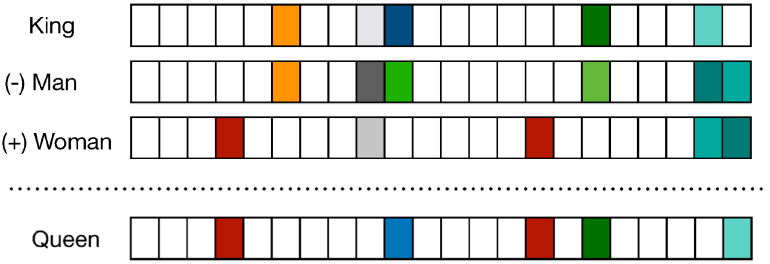
\includegraphics[width=0.55\linewidth]{distributed_representation.png}\\

\textbf{Words to Vectors}

Mathematical function maps word to high dimensional Vector and in neural networks, this function is implemented in the \textcolor{blue}{Embedding Layer} \\

\textbf{Advantage (of vectors)}
\begin{itemize}
    \item Good embedding maps similar/related words to similar regions of the vector space (nearby words have a \textcolor{blue}{semantic similarity})
    \item Dot-Product (Skalarprodukt) is a measure of similarity
    \item Possible to add/subtract vectors
\end{itemize}
\vspace{10pt}
\textbf{Cosine Similarity}

Calculate Similarities between two words (vectors)

\begin{minipage}[t]{0.4\linewidth}
    \vspace{0pt}
    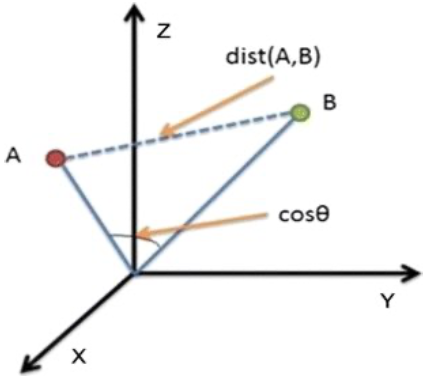
\includegraphics[width=0.8\linewidth]{cosine_distance-1.png}
\end{minipage}
\begin{minipage}[t]{0.6\linewidth}
    cat: A, dog: B \\

    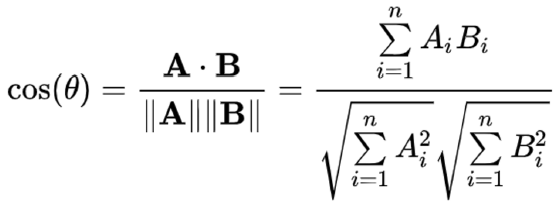
\includegraphics[width=\linewidth]{cosine_distance-formula.png}
\end{minipage}
\vspace{10pt}
\textcolor{blue}{Skalarprodukt (Dot-Product)}

A simplified variant with normalized vectors!

$\mathbf{a} \cdot \mathbf{b} = \sum_{i=1}^n a_i * b_i$ \\

\begin{itemize}
    \item \textcolor{blue}{maximal} when parallel (0\textdegree), both vectors results in max value 1
    \item \textcolor{blue}{zero} when orthogonal (90\textdegree)
    \item \textcolor{blue}{minimal} (negative) when opposite directions (180\textdegree) both vectors results in max value -1
\end{itemize}
\vspace{10pt}



\textcolor{blue}{Example}

A: (3, 6, 2, 1), B: (2, 7, 2, 0)

$A \cdot B = 6 + 42 + 4 + 0 = 52$

$|| A || || B || = \sqrt{(9 + 36 + 4 + 1)} * \sqrt{(4 + 49 + 4 + 0)} = 53.38539$

$\frac{A * B}{( || A || || B ||)} = 0.9740$

$\rightarrow$ high value equals high similarity (to be an animal) \\

\textbf{Cosine Distance}

$cosine distance = 1 - cosine similarity$ \\

\textbf{Magnitude}

Länge eines Vektors

$||A|| = \sqrt{\sum_{i=1}^n A^{2}_i}$
